\documentclass[a4paper,12pt]{article} % Tipo de documento y tamaño de letra.
\usepackage[utf8]{inputenc} % Para que reconozca caracteres especiales como tildes.
\usepackage[spanish]{babel} % Para definir el idioma y el formato de fechas en español.
\usepackage{amsmath, amssymb} % Paquetes para símbolos y ecuaciones avanzadas (Para hacer una ecuación con un recuadro).
\usepackage{ragged2e} % Para justificar textos.
\usepackage{multicol} % Para crear columnas.
\usepackage{slashed} % Para generar números o variables canceladas (Una línea diagonal sobre el número o variable).
\usepackage{graphicx} % Paquete para poner graficas.
\usepackage{float} % Para poder dejar la imagen en un punto fijo del documento.
\usepackage{longtable} % Para tablas largas.
\usepackage{cancel} % Para hacer cancelaciones en medio de operaciones.
\usepackage{xcolor} % Para el color y esas cosas.
\usepackage{apacite} % Paquete para citas APA.
\usepackage{fancyhdr} % Para personalizar encabezados y pies de página.
\usepackage{geometry} % Para ajustar márgenes.
\usepackage{setspace} % Para ajustar el interlineado.
\usepackage{natbib} % Para manejar las citas y que no queden pegadas y feas :P.
\usepackage{hyperref} % Para que los enlaces funcionen con su URL.
\usepackage[version=4]{mhchem}  % Versión recomendada para mayor funcionalidad.
\usepackage{chemfig} %También para hacer estructuras químicas.
\usepackage{array} % Para mejor control de las columnas.
\usepackage{siunitx} % Para unidades físicas.


\pagestyle{fancy}
\fancyhf{} % Limpia encabezados y pies de página predeterminados
\fancyhead[L]{\textbf{ESTADÍSTICA INFERENCIAL.}} % Encabezado izquierdo
\fancyhead[R]{\textbf{ESTADÍSTICA.}} % Encabezado derecho
\fancyfoot[C]{\thepage} % Número de página en el centro del pie

\geometry{headheight=12.96115pt, top=1in, bottom=1in, left=1in, right=1in}
\begin{document}

\begin{figure}[H] 
    \centering
    
\includegraphics[width=0.5\textwidth]{Unir.jpg} 
\end{figure}

\vspace{\baselineskip}

% Ajustamos manualmente todo ;)
\begin{center}
    \textbf{\Large } \\[0.3cm]
    \vspace{\baselineskip}
    \textbf{Liz Ángel Núñez Torres} \\[0.4cm]
    \textbf{Grado en Física} \\[0.4cm]
    \textbf{Universidad Internacional de La Rioja} \\[0.4cm]
    \textbf{29 de Marzo de 2025}
\end{center}



\newpage

\tableofcontents

\newpage


\section*{Pautas de elaboración.}
\addcontentsline{toc}{section}{Introducción}

\vspace{\baselineskip}

\begin{enumerate}
    \item Una breve descripción sobre qué son y para qué se utilizan los \textit{contrastes de hipótesis} (puedes/debes citar la literatura pertinente).

    \item Proponer un algoritmo general que describa cómo se hacen los contrastes de hipótesis a nivel de una población.

    \item Discutir los parámetros que se calculan como parte de este algoritmo.

    \item A continuación, elegir \textbf{dos escenarios modelo} para mostrar cómo puede usarse un contraste de hipótesis para buscar ``respuesta'' a un ``problema'' en el estudio de una población. Esos escenarios/problemas deben estar relacionados con situaciones físicas que definas.

    \item Los modelos deben contener información como:
    \begin{itemize}
        \item Planteamiento del problema (\textbf{dos}).
        \item Definición del tipo de información que recoger para tener la base de datos apropiada en cada caso.
        \item Análisis de cada uno de los estadísticos posibles a analizar y posibles ventajas o desventajas asociadas a su uso (se sugiere se responda a esta cuestión en una tabla).
        \item Presentar los posibles métodos de contraste de hipótesis a utilizar y analizar el impacto de cada uno tomando en cuenta los parámetros a incluir, el coste numérico u otro elemento que consideres relevante a la hora de decidir por una u otra metodología.
    \end{itemize}

    \item Indica claramente qué tipo de conclusiones esperas obtener en cada uno de los escenarios planteados.
\end{enumerate}

\vspace{\baselineskip}


\section{Contrastes de hipótesis.}

\begin{justify}
Los contrastes de hipótesis son métodos estadísticos que determinan a un cierto nivel de significación, para qué valores de la muestra se rechaza o no la hipótesis.
\end{justify}
\begin{justify}
    Se utilizan para denotar una región crítica o de rechazo \textit{(RC)} y una región de aceptación \textit{(RA)}. \cite{Introductory-statistics}
\end{justify}

\vspace{\baselineskip}

\section{Algoritmo.}

\begin{justify}
    El \textbf{algoritmo} a proceder es:
\end{justify}

\begin{enumerate}
    \item Formular lal hipótesis.
    \item Seleccionar el nivel de significancia \( \alpha.\)
    \item Elegir el estadístisco de adecuado (Normal, T-student, etc).
    \item Calcular el estadístico de prueba \(Z \; \text{o} \; t\).
    \item Determinar la región crítica o el valor-p.
    \item Tomar la decisión (Rechazar o no \(H_0\)).
    \item Conlusión contextual.
\end{enumerate}

\vspace{\baselineskip}

\section{Parámetros del algoritmo.}

\vspace{\baselineskip}

\begin{justify}
    Usaremos los siguientes parámetros para desarrollar el contraste hipotético,
    donde el funcionamiento de los mismo vendrá a cabo por el tipo de estadístico de prueba. 
\end{justify}

\vspace{\baselineskip}

\begin{multicols}{2}
    \(1) \; \tilde{x} =\) Promedio de la muestra. 

    \(5) \; gl = \) Grado de libertad.
\end{multicols}

\begin{multicols}{2}
    \(2)\; \alpha = \) nivel de significancia
    
    \(6)\) Valor \(p =\) Probabilidad del resultado.
\end{multicols}

\begin{multicols}{2}
    \(3)\; s \; \text{o} \; \sigma =\) Desviación estándar.

    \(7) \; H_0 \Rightarrow (RC,RA) =\) región de rechazo.
    
\end{multicols}

\begin{multicols}{2}
    \(4) \; (Z,t =)\) Estadístico de prueba.

    \(8) \; (p > \alpha)\; \text{o} \; (p < \alpha) =\) Decisión.
\end{multicols}

\vspace{\baselineskip}

\section{Escenarios modelo.}

\begin{enumerate}
    \item Un biólogo desea verificar si el tamaño promedio de las carpas en un embalse de aragón es diferente 
    al de otros embalses, que es de \(22 \; cm\). Toma una muestra de 20 carpas, obtiene una media de 23.58 \(cm\)
    y una desviación estandar de 4.3. ¿Hay evidencia para afirmar que las carpas de este embalse son más grandes con un 95\% de confianza?

    \item Una fábrica afirma que el contenido medio de azúcar por bebida es de \(30 \; g\). Se toma una muestra aleatoria de 100 bebidas,
    con una desviación estándar de \(5 \; g\). La media muestral obtenida es de 28.9 ¿Es correcta esta afirmación con un nivel de confianza del 95\%?
\end{enumerate}


\section{Desarrollo de los modelos.}
\vspace{\baselineskip}


\begin{table}[H]
\centering
\resizebox{\textwidth}{!}{
\begin{tabular}{|c|c|c|c|}
\hline
\textbf{Estadístico} & \textbf{Uso recomendado} & \textbf{Ventajas} & \textbf{Desventajas} \\
\hline
\textbf{Z} & $\sigma$ conocida y $n \geq 30$ & Cálculos sencillos, tabla normal estándar & Requiere conocer $\sigma$ \\
\hline
\textbf{t} & $\sigma$ desconocida y/o $n < 30$ & Más flexible para muestras pequeñas & Requiere estimar varianza \\
\hline
\end{tabular}
}
\end{table}

\begin{justify}
    Con la información obtenida del cuadro y los datos suministrados por los \textbf{escenarios modelo} procedemos a dar respuesta.
\end{justify}

\begin{itemize}
    \item \textbf{El problema 1, tamaño de carpas,} lo haremos con \textbf{T-Student} porque \(\sigma\) es desconocida y \(n < 30 \).
    \item \textbf{El problema 2, fábrica,} lo haremos con \textbf{Z-Normal} porque \(\sigma\) es conocida y \(n > 30\).
\end{itemize}

\subsection{Carpas  T-Student.}

\begin{enumerate}
    \item Hipotesis.
    
    \[H_0: \mu = 22 \;\;\;\;\;\;\; \text{Las carpas no son más grandes.}\]
    \[H_1: \mu > 22 \;\;\;\;\;\;\; \text{Las carpas son más grandes.}\]

    \item Elegir estadístico: Lo hemos hecho antes, T-Student.

    \item Nivel de significancia.
    \[ \alpha = 0.05\]

    \item Estadistico.
    \[t = \frac{\tilde{x} - \mu_0}{s/\sqrt{n}} \Rightarrow \frac{23.58 - 22}{4.3/\sqrt{20}} = \frac{1.58}{0.9615} = 1.643\]

    \item Valor-p y región crítica.
    \begin{itemize}
        \item Los grados de libertad son \(df = n -1 = 19.\)
        \item Con \(\alpha = 0.05\) y contraste \textbf{unilateral (cola derecha)} el valor crítico (evaluado con \(R\)) es \(t_{crit}= 1.729\).
    \end{itemize}

    \item Tomar decisión.
    \[t < t_{crit} \Rightarrow 1.643 < 1.729.\]

    \textbf{No se rechaza \(H_0\).}

    \item Conclusión.
    \begin{justify}
        \textbf{No hay suficiente evidencia estadística, al 95\% de confianza, para afirmar que las carpas de este embalse son más grandes que las de otros embalses.}
    \end{justify}
\end{enumerate}

\subsection{Fábrica Z(Normal).}

\begin{enumerate}
    \item Hipótesis.
    \[H_0: \mu = 30\]
    \[H_1: = \mu \neq 30 \; \text{(Bilateral.)} \]

    \item Elegir estadístico: Lo hemos hecho antes, Z(Normal).

    \item Nivel de significancia \(\alpha = 0.05 \)
    
    \item Estadístico.
    \[Z = \frac{\tilde{x} - \mu_0}{\sigma / \sqrt{n}} \Rightarrow \frac{28.9 - 30}{5 / \sqrt{100}} = \frac{-1.1}{0.5}= -2.2\]

    \item Valor p y región crítica.
    \begin{itemize}
        \item \(p = 2 \times P (Z <  -2.2) = 2 \times 0.0139 = \) \textbf{0.0278}.
        \item En un contraste bilateral, donde la región está en las dos colas. 
        \[\alpha = 0.05 \Rightarrow Z_{\alpha/2} = 0.025 = \pm 1.96 \; \text{(evaluado con R)} \].
    \end{itemize}
    \item Tomar decisión
        
        \[2.2 > 1.96 \Rightarrow \; \text{Rechazamos} \; H_0.\]
        \[p < \alpha = 0.0278 < 0.05 \Rightarrow \; \text{Rechazamos} \; H_0.\]

    \item Conclusión.

    \begin{justify}
        \textbf{No hay evidencia suficiente para apoyar la afirmación de la fábrica, no con un 95\% de confianza.}
    \end{justify}
\end{enumerate}

\section{Conclusiones que esperabamos obtener de los escenarios.}

\subsection{Carpas.}

\begin{justify}
    Esperabamos que no hubiese evidencia contra \(H_0\) debido al tamaño de muestra pequeño y la alta variabilidad \(s = 4.3 \; cm\) aunque la media fuese de \( 1.58 \; cm\) más grande que la esperada.
\end{justify}

\subsection{Fábrica.}
\begin{justify}
    Esperabamos un resultado similar al modelo anterior, esto debido que la diferencia entre \(\tilde{x}= 28.9\) y \(\mu = 30\) es una leve diferencia de \textbf{-1.1 g},
    en una muestra muy grande \(n = 100\).
\end{justify}
\newpage

% Aquí ajustamos y usamos las referencias y citas del archivo .bib.
\setlength{\bibsep}{12pt} % Ajusta la separación entre referencias
\bibliographystyle{apacite} % Estilo APA
\bibliography{citas} % Archivo de referencias

\section{Calificación/Observaciones.}

\begin{figure}[H]
    \centering
    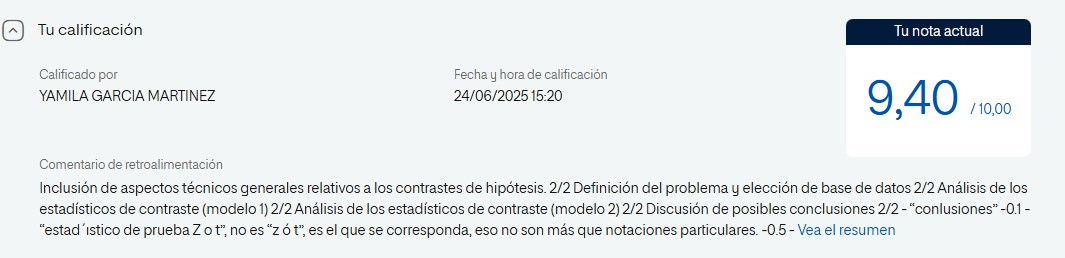
\includegraphics[width=1 \textwidth]{calificacion.jpg}
\end{figure}

\end{document}